% PLOS manuscript prepared for Overleaf
% Based on the PLOS LaTeX template, version 3.6 (August 2022), and current PLOS ONE submission guidance.
% Compile with pdfLaTeX -> BibTeX -> pdfLaTeX -> pdfLaTeX.
\documentclass[10pt,letterpaper]{article}
\usepackage[top=0.85in,left=2.75in,footskip=0.75in]{geometry}
\usepackage[T1]{fontenc}
\usepackage[utf8]{inputenc}
\usepackage{amsmath,amssymb}
\usepackage{changepage}
\usepackage{textcomp,marvosym}
\usepackage{cite}
\usepackage{nameref,hyperref}
\usepackage[right]{lineno}
\usepackage[nopatch=eqnum]{microtype}
\DisableLigatures[f]{encoding = *, family = *}
\usepackage[table]{xcolor}
\usepackage{array}
\usepackage{longtable,tabularx,booktabs}
\usepackage{setspace}
\usepackage[aboveskip=1pt,labelfont=bf,labelsep=period,justification=raggedright,singlelinecheck=off]{caption}
\usepackage{lastpage,fancyhdr,graphicx}
\usepackage{epstopdf}

% PLOS manuscript layout
\doublespacing
\raggedright
\setlength{\parindent}{0.5cm}
\textwidth 5.25in
\textheight 8.75in
\renewcommand{\figurename}{Fig}
\bibliographystyle{plos2015}
\makeatletter
\renewcommand{\@biblabel}[1]{\quad#1.}
\makeatother

% Header and footer
\pagestyle{fancy}
\fancyhf{}
\rfoot{\thepage/\pageref{LastPage}}
\renewcommand{\headrulewidth}{0pt}
\renewcommand{\footrule}{\hrule height 2pt \vspace{2mm}}
\fancyheadoffset[L]{2.25in}
\fancyfootoffset[L]{2.25in}
\lfoot{Draft manuscript}
\hypersetup{hidelinks}

% Review-copy switch. Keep true for convenient Overleaf rendering.
% Change to \showfiguresfalse for the PLOS initial-submission manuscript PDF,
% because PLOS asks authors to upload the figure files separately.
\newif\ifshowfigures
\showfigurestrue

\begin{document}
\vspace*{0.2in}
\begin{flushleft}
{\Large\textbf{Reconstructing individual patient data from published Kaplan--Meier curves: A systematic methodological review and practical guide}}
\\[12pt]
\textit{[Author names]}\\[8pt]
\textbf{1} [Department/Program/Center, Institution, City, State/Province, Country]\\
\textbf{2} [Department/Program/Center, Institution, City, State/Province, Country]\\[8pt]
* [Corresponding author email]\\[12pt]
\textbf{Short title:} Reconstruction of survival IPD from Kaplan--Meier curves
\end{flushleft}
\clearpage
\section*{Abstract}

Time-to-event outcomes are central to clinical trials, evidence synthesis, and health-economic evaluation, but published reports commonly provide only hazard ratios, selected survival summaries, and Kaplan--Meier curves. The underlying individual patient data are often unavailable because of privacy, proprietary, regulatory, and logistical restrictions. This review identified and classified methods and software for digitizing published Kaplan--Meier curves and reconstructing patient-level survival time and event status. Searches of PubMed, Google Scholar, arXiv, and the Comprehensive R Archive Network identified 698 records; after the prespecified source cap, deduplication, screening, and full-text assessment, 15 reports were retained and mapped to 11 method or tool entities. The evidence was organized into foundational algorithms, implementations, core reconstruction methods, upstream digitization or automation, downstream extensions, and evaluation studies. IPDfromKM, KMtoIPD, and the CEN-KM component of RESOLVE-IPD were retained as the three core reconstruction approaches because each provides distinct reconstruction logic, a runnable implementation, and patient-level time-to-event output. Their practical suitability depends mainly on the availability of a risk table, the visibility and overlap of censoring marks, the presence of an editable vector source, and the acceptable implementation burden. Other tools serve primarily as implementations, digitizers, automated interfaces, or extensions for subgroup and covariate reconstruction. The resulting framework separates methodological novelty from software packaging and provides a reproducible decision pathway for selecting, validating, and documenting a Kaplan--Meier-to-IPD workflow.

\linenumbers

\section*{1. Introduction}

Time-to-event outcomes are widely used when the timing of death, disease progression, recurrence, treatment discontinuation, or another clinical event is more informative than whether the event occurred alone. In systematic reviews and meta-analyses, these outcomes are commonly synthesized with hazard ratios because they incorporate both event timing and censoring, while Kaplan--Meier (KM) curves provide the principal graphical summary of the observed survival experience \cite{tierney2007}. The same information is also central to trial planning, comparative-effectiveness research, and health-economic models that require survival over a clinically relevant horizon.

Published summary measures do not preserve all of the information needed for secondary survival analysis. A hazard ratio is tied to the proportional-hazards framework and may be difficult to interpret when treatment effects change over time. Median survival uses only one point on the survival distribution, and many reports omit alternative estimands such as fixed-time survival probabilities or restricted mean survival time (RMST). RMST, defined by the area under the survival curve up to a prespecified time, can provide a clinically interpretable treatment contrast without requiring proportional hazards \cite{royston2013}. Patient-level time and event data also permit reassessment of proportional hazards, flexible parametric modeling, estimation of alternative treatment effects, and analyses that cannot be recovered from a single published summary \cite{guyot2012,wei2017}.

Individual patient data (IPD) meta-analysis can support harmonized outcome definitions, consistent analysis across studies, and detailed assessment of participant- and study-level variation. In practice, however, original trial IPD are frequently inaccessible. Privacy protections, proprietary ownership, data-use agreements, regulatory constraints, and the resources required to curate and share trial data can all prevent direct access \cite{liu2021,kim2025}. This creates a recurrent gap between the analyses that are scientifically desirable and the information that is publicly available.

Published KM figures preserve part of the missing information. Their step functions encode event times and changes in survival probability; risk tables provide intermittent constraints on cohort attrition; total event counts and plotted censoring symbols may add further information. Reconstruction methods reverse this reporting process by first converting the figure into structured coordinates and then assigning event and censoring times so that the reconstructed patient-level data reproduce the published curve and accompanying summaries. The iterative algorithm introduced by Guyot et al.~established the main reconstruction framework and showed that accuracy improves when numbers at risk or total event counts are available \cite{guyot2012}. Later implementations improved preprocessing, usability, numerical stability, treatment of observed censoring marks, and automation \cite{wei2017,liu2021,rogula2022,zhang2024}.

The resulting literature is difficult to interpret as a simple catalogue of software. A foundational algorithm may appear as author code, a package, a command in another language, and a later wrapper without representing four independent statistical methods. Conversely, recent systems may add a genuinely different reconstruction strategy, automate only the digitization stage, or target a downstream problem such as complementary-subgroup recovery, covariate generation, or uncertain subgroup labels \cite{zhao2022,kmgpt2025,synthipd2026,resolve2026}. Validation also differs across studies, ranging from known simulated IPD to agreement with published summary measures, making published accuracy statistics unsuitable for an unqualified ranking.

This study therefore conducted a systematic methodological review of KM digitization, KM-to-IPD reconstruction, and closely related extensions. Section 2 describes the search, eligibility criteria, evidence classification, and report-to-entity mapping. Section 3 compares the inputs, reconstruction logic, outputs, validation evidence, and implementation constraints of the three core reconstruction approaches. Section 4 converts these findings into a practical guide for selecting a method, validating the reconstructed data, and preserving a reproducible analysis record.

\section*{2. Systematic review methods and evidence structure}

\subsection*{2.1 Review design}

This systematic methodological review identified and compared methods, software implementations, and extensions for extracting information from published KM curves and reconstructing time-to-event IPD. The review is reported in accordance with PRISMA 2020, with the completed checklist provided as S1 Checklist \cite{page2021}. Because the included evidence did not estimate a common intervention effect, findings were synthesized narratively rather than statistically pooled.

\subsection*{2.2 Review questions, eligibility criteria, and units of analysis}

The review addressed three linked questions: which reports proposed or evaluated KM-specific digitization, KM-to-IPD reconstruction, censor-identification, or post-reconstruction extension methods; which independent method or tool entities those records represented; and how the entities differed in required inputs, reconstruction logic, censoring treatment, outputs, diagnostics, platform, and reproducibility.

Eligible records included original reports proposing a KM-specific digitization, time-to-event reconstruction, censor-identification, or reconstruction extension method; software packages, commands, web applications, or research code with sufficient documentation to reproduce the central workflow; and substantive validation studies. Application papers that only used reconstructed IPD, generic graph digitizers without a KM-specific contribution, narrative reviews without new validation, and records lacking sufficient technical information were excluded. Publications, packages, web applications, and code repositories were treated as report or software records. Multiple records could map to one method or tool entity, while sequential outputs from the same research group were retained separately when they introduced materially different reconstruction logic or targets.

\subsection*{2.3 Information sources, screening, and data extraction}

PubMed, Google Scholar Advanced, arXiv, and the Comprehensive R Archive Network were searched on 24 May 2026 for records published from 2012 onward. PubMed used three complementary concept groups covering IPD reconstruction, curve digitization or automation, and method validation. Google Scholar used four advanced-search combinations with relevance sorting, while arXiv and the Comprehensive R Archive Network were used to identify preprints and software records. Complete search strings, settings, source limits, and returned counts are provided in S1 Table.

The ten logged searches returned 698 records. One Google Scholar query returned 345 results, of which the first 200 relevance-ranked records were designated for screening; 145 returned results therefore remained outside the screening set. After this source-level cap, 553 records were designated for deduplication and screening. Records were deduplicated using bibliographic identifiers and normalized titles, screened against the prespecified eligibility criteria, and assessed in full text. For eligible records, extraction covered the target task, required figure and structured inputs, use of risk tables, total events and censor marks, digitization route, reconstruction algorithm, outputs, diagnostic measures, platform, implementation status, validation design, and reported limitations. Report-to-entity mapping was performed after eligibility assessment so that papers, packages, interfaces, and wrappers sharing one methodological core were not counted as separate methods.

\subsection*{2.4 Evidence classification and study selection}

The evidence was organized into six functional layers: foundational algorithms, implementation records, core reconstruction methods, upstream digitization or end-to-end automation, downstream extensions, and evaluation or contextual evidence. Core reconstruction was defined as the conversion of structured KM-derived information into patient-level records containing at least survival time and event status. This classification separated methodological novelty from software packaging and defined the analytic role of each included entity (Table~\ref{tab:evidence}).

\begin{table}[!ht]
\begin{adjustwidth}{-2.25in}{0in}
\centering
\caption{\textbf{Evidence layers and analytic disposition.}}
\label{tab:evidence}
\begin{nolinenumbers}
\begingroup
\setstretch{1.05}
\setlength{\tabcolsep}{3pt}
\renewcommand{\arraystretch}{1.25}
\footnotesize
\begin{tabular}{|>{\raggedright\arraybackslash}p{1.10in}|>{\raggedright\arraybackslash}p{1.48in}|>{\raggedright\arraybackslash}p{2.15in}|>{\raggedright\arraybackslash}p{2.05in}|}
\hline
\rowcolor{gray!18} \textbf{Layer} & \textbf{Representative entities} & \textbf{Defining contribution} & \textbf{Treatment in the review} \\ \hline
Foundational algorithm & Guyot/iKM & Original iterative reconstruction logic using digitized Kaplan--Meier coordinates and reported risk-set information. & Retained as the methodological baseline; not presented as a current standalone package. \\ \hline
Implementation layer & ipdfc; survHE; reconstructKM & Operational implementations or workflow packaging of Guyot/iKM and closely related reconstruction steps. & Described narratively as platform and workflow choices; not counted as independent method families. \\ \hline
Core reconstruction & IPDfromKM; KMtoIPD; CEN-KM/RESOLVE-IPD & Distinct arm-level reconstruction logic with a runnable implementation and patient-level time and event output. & Compared directly in Section 3 and Table 2. \\ \hline
Upstream digitization and automation & SurvdigitizeR; KM-GPT & Automated coordinate extraction or end-to-end image processing around a reconstruction core. & Included as workflow options, but not automatically treated as new statistical reconstruction methods. \\ \hline
Downstream extensions & KMSubtraction; SynthIPD; MAPLE & Recovery of complementary subgroups, generation of covariate-rich synthetic data, or propagation of subgroup-label uncertainty. & Discussed separately because the target differs from standard arm-level time-to-event reconstruction. \\ \hline
Evaluation and context & Kim et al. (2025) & Practical validation or comparison of existing reconstruction workflows. & Used to interpret accuracy and implementation evidence; not counted as a new method. \\ \hline
\end{tabular}
\endgroup
\end{nolinenumbers}
\end{adjustwidth}
\end{table}

\emph{Note:} Classification is based on functional contribution and reconstruction target rather than author overlap.

% PLACEHOLDER PRISMA COUNTS: replace after the updated search and ledger audit.
After the source-level cap, 553 records entered deduplication. Twenty-seven duplicates were removed, leaving 526 records for title and abstract screening. Of these, 507 were excluded and 19 reports were assessed in full text. Four reports were excluded because they were application-only reports (n = 2), were not specific to KM digitization or reconstruction (n = 1), or lacked sufficient technical documentation (n = 1). Fifteen reports were included and mapped to 11 method or tool entities. The study-selection sequence is shown in Fig~\ref{fig:prisma}.

\begin{figure}[!ht]
\centering
\ifshowfigures
\fbox{\parbox[c][2.0in][c]{0.92\textwidth}{\centering\textbf{Draft placeholder: Fig 1}\\[4pt]Replace this box with the final PRISMA 2020 flow diagram after the screening ledger is audited.}}
\fi
\caption{\textbf{PRISMA 2020 flow diagram for identification, screening, eligibility assessment, and inclusion.} Report-level counts are shown through full-text inclusion; mapping to method and tool entities was performed after eligibility assessment.}
\label{fig:prisma}
\end{figure}

\subsection*{2.5 Boundary of the core comparison}

The Guyot/iKM algorithm was retained as the methodological baseline, while ipdfc, survHE, and reconstructKM were treated as implementation records because they operationalize the same foundational reconstruction family in different languages or broader workflows \cite{guyot2012,wei2017,baio2020,reconstructkm2025}. SurvdigitizeR was retained as an upstream digitization tool because it returns curve coordinates rather than patient-level event histories \cite{zhang2024}. KM-GPT was treated as an end-to-end automation system whose reconstruction stage remains based on an adapted iKM core \cite{kmgpt2025}. KMSubtraction, SynthIPD, and MAPLE address complementary-subgroup recovery, covariate-rich synthetic data, or subgroup-label uncertainty and therefore target questions beyond standard arm-level reconstruction \cite{zhao2022,synthipd2026,resolve2026}. These tools remain relevant to the overall workflow but were not included in the direct comparison of independent arm-level reconstruction logics.

\section*{3. Functional analysis of reconstruction methods}

\subsection*{3.1 Scope and core methods}

The functional analysis compared capabilities documented in peer-reviewed articles, preprints, software records, public repositories, and web documentation available through 13 August 2026. A method entered the core comparison when it had a distinct and explainable reconstruction logic, sufficient technical detail, a publicly runnable implementation, and a primary output containing patient-level survival time and event status. IPDfromKM, KMtoIPD, and CEN-KM within RESOLVE-IPD met these criteria. Guyot/iKM remained the baseline, while implementations, digitizers, automated interfaces, and downstream extensions were analyzed in their respective layers. Table~\ref{tab:core-methods} summarizes the features that directly determine how the three core methods can be used.

\begin{nolinenumbers}
\begingroup
\setstretch{1.03}
\setlength{\tabcolsep}{3pt}
\renewcommand{\arraystretch}{1.22}
\footnotesize
\setlength{\LTleft}{-2.22in}
\setlength{\LTright}{0in}
\begin{adjustwidth}{-2.22in}{0in}
\captionof{table}{\textbf{Core reconstruction methods.}}\label{tab:core-methods}
\end{adjustwidth}
\begin{longtable}{|>{\raggedright\arraybackslash}p{1.00in}|>{\raggedright\arraybackslash}p{1.98in}|>{\raggedright\arraybackslash}p{1.98in}|>{\raggedright\arraybackslash}p{2.05in}|}
\hline
\rowcolor{gray!18} \textbf{Domain} & \textbf{IPDfromKM} & \textbf{KMtoIPD} & \textbf{CEN-KM / RESOLVE-IPD} \\ \hline
\endfirsthead
\multicolumn{4}{l}{\footnotesize\textit{Table \thetable\ continued from the previous page.}}\\
\hline
\rowcolor{gray!18} \textbf{Domain} & \textbf{IPDfromKM} & \textbf{KMtoIPD} & \textbf{CEN-KM / RESOLVE-IPD} \\ \hline
\endhead
\hline
\multicolumn{4}{r}{\footnotesize\textit{Continued on the next page.}}\\
\endfoot
\hline
\endlastfoot
Primary target & Arm-level time-to-event IPD from a published Kaplan--Meier curve. & Arm-level time-to-event IPD from observed survival drops and, when available, marked censoring times. & Arm-level time-to-event IPD within a broader vector-extraction and subgroup-analysis framework. \\ \hline
Recommended input & Digitized time-survival coordinates, baseline cohort size, and interval-specific numbers at risk; total events may be added. & Total sample size and lower coordinates of survival drops; digitized censoring times are optional but central when no risk table is available. & Sample size, event/drop times, survival probabilities, and optional censoring times; VEC-KM additionally requires an eligible vector PDF or SVG. \\ \hline
Risk table & Strongly recommended because interval-specific risk sets constrain inferred censoring counts. & Not required. & Optional in the documented reconstruction core; current risk-table alignment remains less mature than the vector/censor route. \\ \hline
Censor information & Censoring is inferred within risk-table intervals rather than treating each plotted mark as an observed censoring time. & Digitized censoring times can be inserted directly; ambiguous or overlapping marks remain a source-figure limitation. & Explicit and duplicate censoring times can be represented while candidate allocations are evaluated against the target curve. \\ \hline
Digitization route & Interactive point acquisition in the R/Shiny workflow or externally digitized coordinates. & External digitization of the lower step coordinates and censor marks. & VEC-KM extracts curves and censor symbols from vector graphics; target-panel identification is still required. \\ \hline
Reconstruction logic & Modified iterative Guyot/iKM algorithm with automated preprocessing and numerical safeguards. & Greedy event allocation at observed Kaplan--Meier drops with optional direct use of censoring times. & CEN-KM branch-and-compare search over censoring configurations, followed by target-curve comparison. \\ \hline
Primary output & Patient-level survival time and event status, reconstructed curve, risk-set comparison, and standard survival summaries. & Patient-level survival time and event indicator. & Patient-level survival time and event indicator; MAPLE can add ensembles of subgroup labels in the broader framework. \\ \hline
Diagnostics & Curve and risk-set comparison with RMSE, MAE, maximum absolute error, Kolmogorov-Smirnov statistic, and survival summaries. & The method paper evaluates curve fit, hazard ratios, and survival quantiles; a standardized package report is not built in. & Target-curve tolerance and refitting checks; research-code outputs require explicit archiving of inputs and settings. \\ \hline
Implementation considerations & Peer-reviewed R package and Shiny workflow; well suited to reproducible local analysis when risk-table information is available. & Peer-reviewed R implementation with a compact workflow; performance depends on reliable identification of drops and censor marks. & Preprint and research-code framework with vector-specific advantages and greater version-control and reproducibility burden. \\ \hline
\end{longtable}
\endgroup
\end{nolinenumbers}

\emph{Note:} The comparison is documentation-based and does not represent a new head-to-head execution benchmark.

\subsection*{3.2 Comparative characteristics, validation, and practical limitations}

IPDfromKM combines interactive coordinate acquisition, automated preprocessing, a modified iKM reconstruction algorithm, and diagnostic summaries in an R package and Shiny workflow \cite{liu2021}. Its recommended inputs are digitized time-survival coordinates, baseline cohort size, and risk-table times with corresponding numbers at risk; a total event count may provide an additional constraint. The risk table is central to the method because interval-specific risk sets constrain the number of inferred censoring observations. Although the algorithm can run with baseline cohort size alone, the censoring pattern is then less identifiable and the reconstruction is more weakly constrained.

KMtoIPD uses the total sample size and the lower coordinates of observed survival drops to allocate event counts and can insert digitized censoring times directly into the patient-level sequence \cite{rogula2022}. It therefore does not require a risk table and is most informative when censoring marks are clearly visible and can be separated from curve steps. Its use of plotted censoring information does not remove ambiguity from the source figure: one mark may conceal multiple censoring events, marks may overlap, and raster compression or multiple curves may prevent reliable assignment.

RESOLVE-IPD separates high-fidelity vector extraction from censoring-informed reconstruction \cite{resolve2026}. VEC-KM extracts curves and censor symbols from eligible vector PDF or SVG content, while CEN-KM evaluates candidate censoring configurations against the target curve through a branch-and-compare procedure. This permits explicit and duplicate censoring times and differs from both risk-table-constrained iKM reconstruction and the adapted-iKM pipeline used by KM-GPT. The method's vector-specific advantages are accompanied by research-code maturity, target-panel identification, and a greater need to freeze versions, parameters, and intermediate files.

All three methods return patient-level survival time and event status. IPDfromKM additionally supplies reconstructed curves, risk-set comparisons, RMSE, MAE, maximum absolute error, a Kolmogorov-Smirnov statistic, and common survival summaries \cite{liu2021}. KMtoIPD returns a compact patient-level dataset; the accompanying study evaluates curve agreement, hazard ratios, and survival quantiles, so a consistent diagnostic report must be constructed around the output \cite{rogula2022}. RESOLVE-IPD uses target-curve tolerance and refitting checks and can add ensembles of plausible subgroup labels through MAPLE, although those label outputs belong to the extension layer rather than the core arm-level reconstruction. Diagnostic thresholds proposed in individual papers were treated as method-specific empirical rules rather than universal acceptance criteria.

Validation evidence differed in target and reference standard. Guyot/iKM, IPDfromKM, and KMtoIPD used simulated data, original IPD, or published summaries to evaluate reconstructed curves and survival estimates \cite{guyot2012,liu2021,rogula2022}. SurvdigitizeR evaluated coordinate extraction rather than the complete patient-level reconstruction \cite{zhang2024}, while the principal evidence for KM-GPT, SynthIPD, and RESOLVE-IPD remained author-led preprint validation at the evidence freeze \cite{kmgpt2025,synthipd2026,resolve2026}. The real-world study by Kim et al.~provided useful external evidence for an existing workflow, but differences in figures, information availability, sample size, censoring, and evaluation metrics prevented a direct cross-method ranking \cite{kim2025}. Simulation evidence was interpreted according to the aims, data-generating mechanisms, estimands, methods, and performance measures reported by each study \cite{morris2019}.

Implementation choices alter the practical workflow without changing the underlying method family. ipdfc provides a peer-reviewed Stata implementation of iKM, survHE embeds reconstruction within a health-economic survival-modeling suite, and reconstructKM supplies R utilities for formatted curve and risk-table inputs \cite{wei2017,baio2020,reconstructkm2025}. Local R, Stata, or Python workflows support versioned scripts and offline archiving, whereas browser and model-assisted systems may introduce service availability, data-transfer, credential, and model-version dependencies. These differences should be recorded as reproducibility characteristics rather than interpreted as evidence of statistical superiority.

Across methods, the most consequential failures arise before or during reconstruction: the wrong curve may be matched to a risk table, axes may be clipped or miscalibrated, censoring symbols may be unobservable, and low-resolution images may prevent reproducible localization of curve steps. The response depends on whether the missing information can be replaced by another reliable constraint. A reconstruction should be revised or abandoned when source identity, calibration, or validation cannot be defended (Fig~\ref{fig:failure}).

\begin{figure}[!ht]
\centering
\ifshowfigures
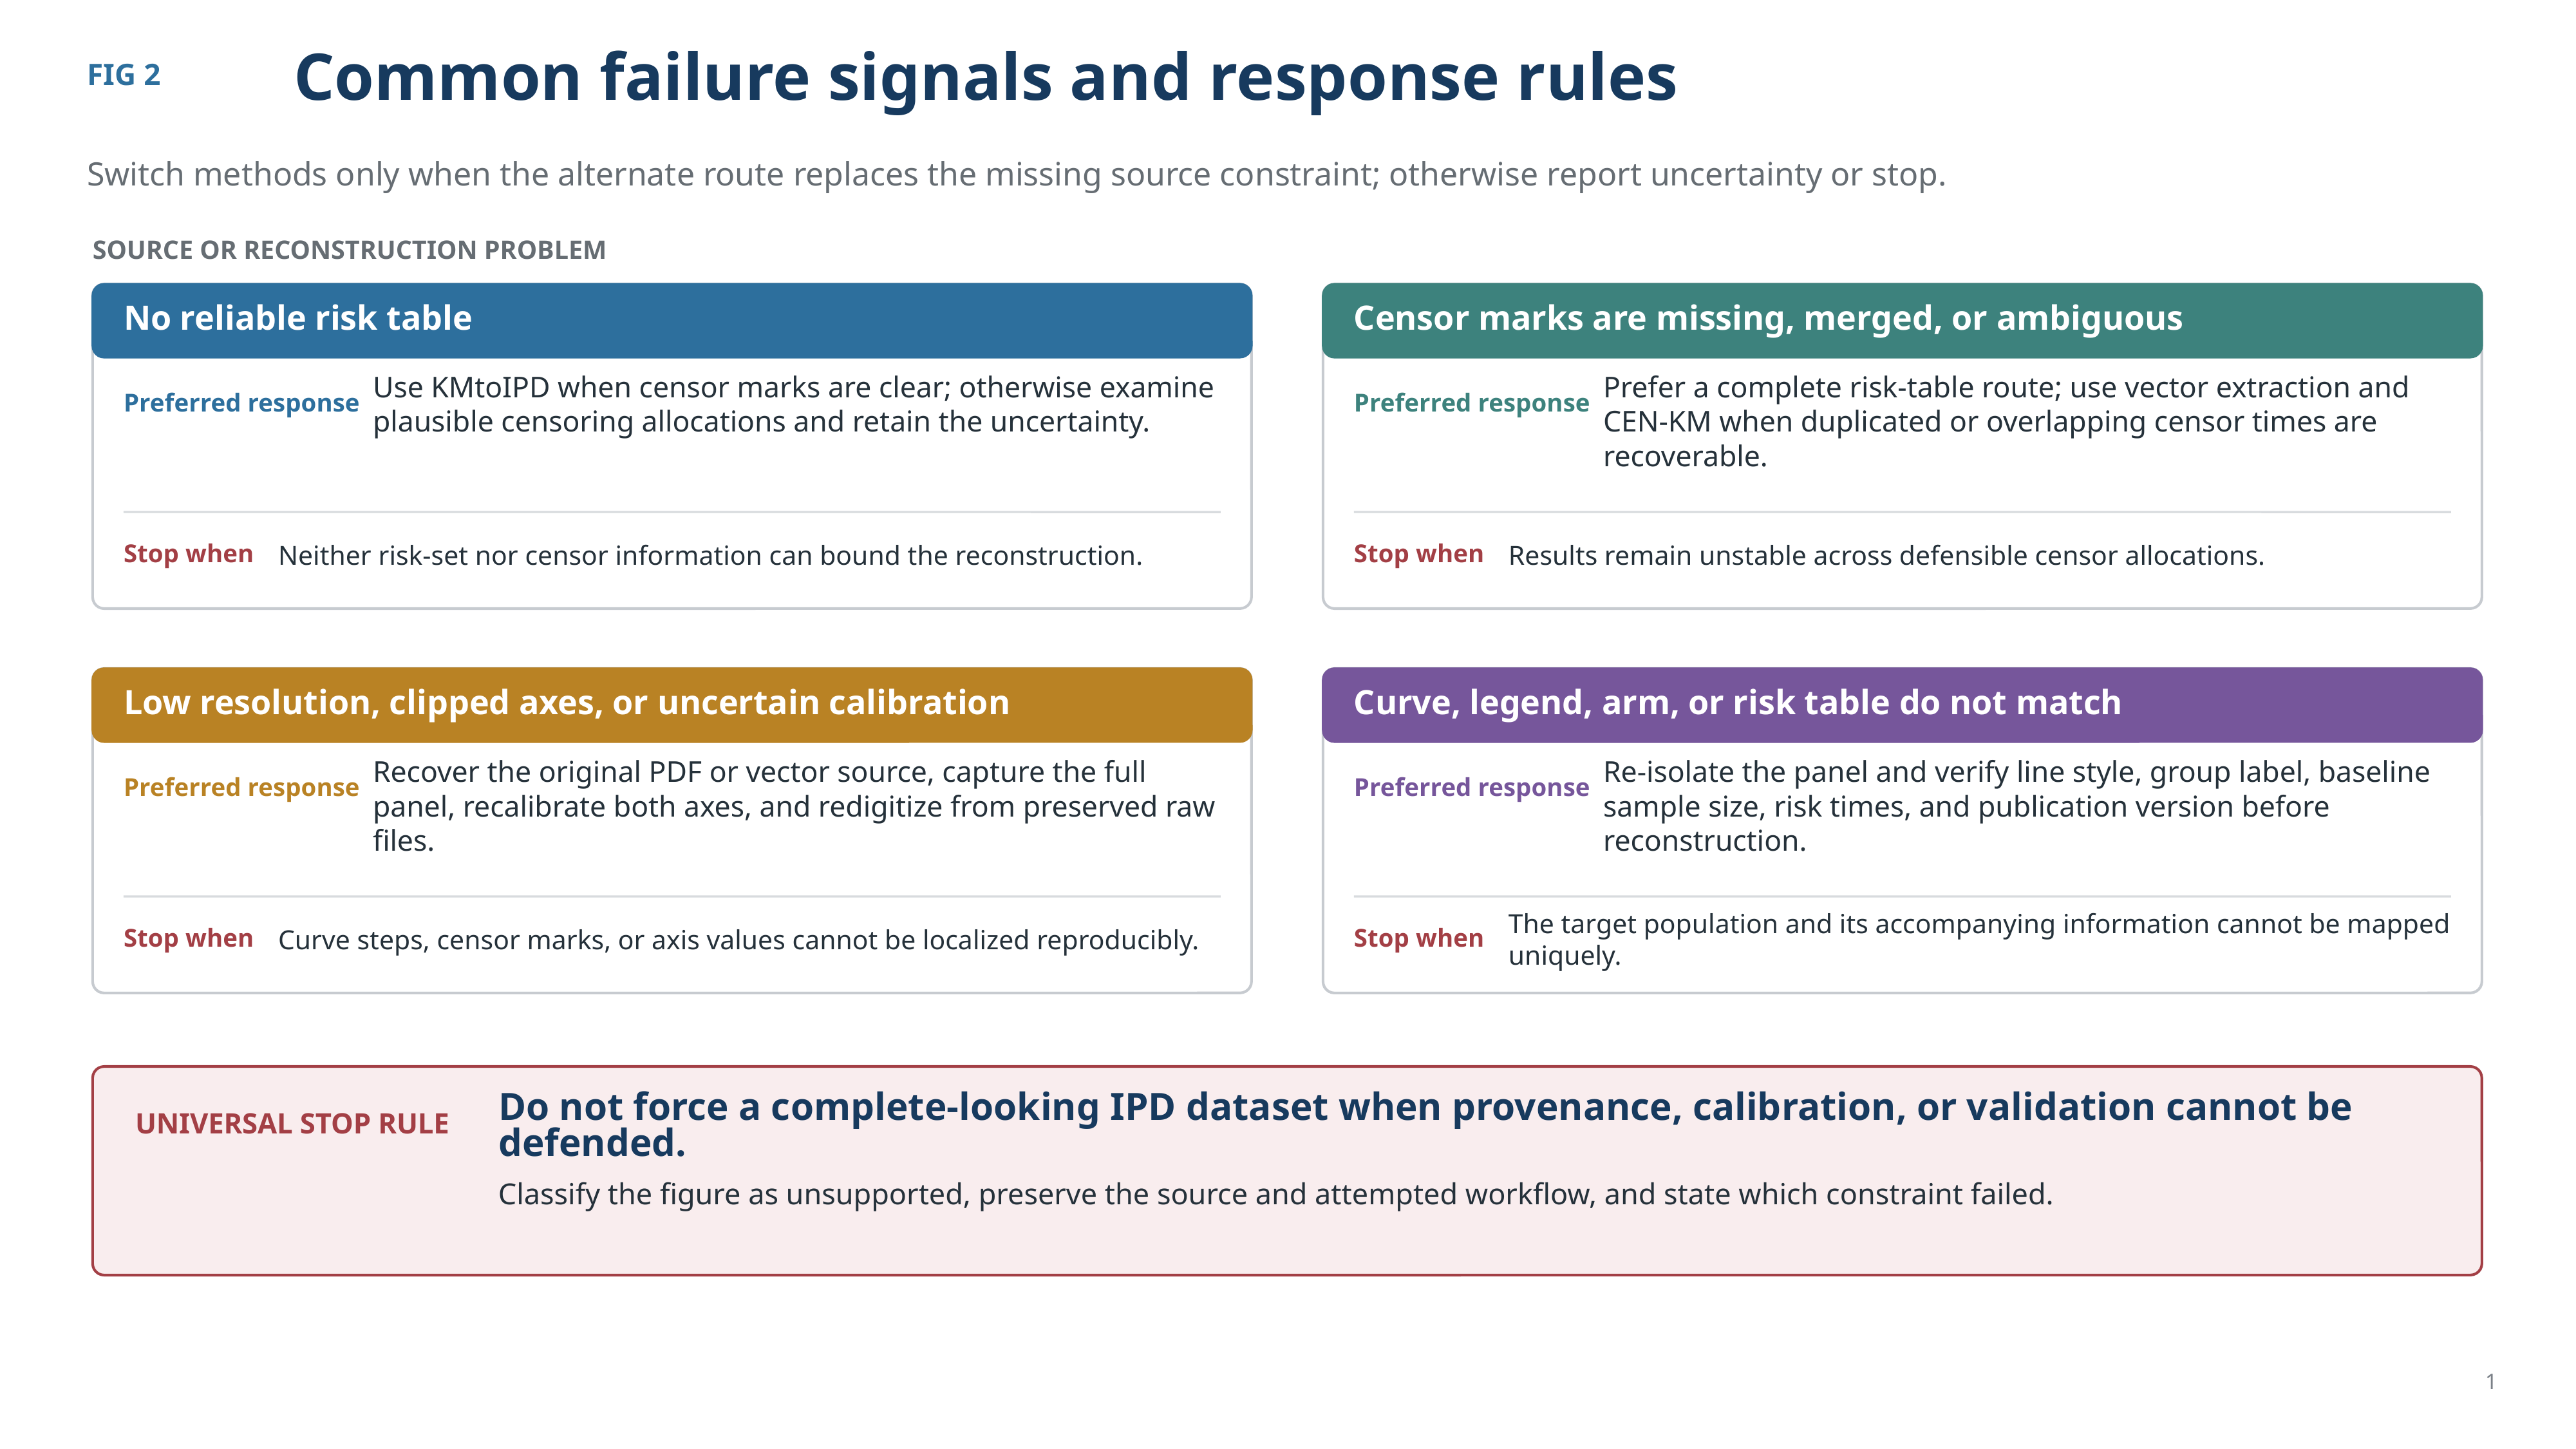
\includegraphics[width=\textwidth]{Fig2.png}
\fi
\caption{\textbf{Common failure signals and response rules for KM-to-IPD reconstruction.} The compact framework links missing risk information, ambiguous censoring, poor image quality, and curve-risk mismatch to an alternative input route, redigitization, sensitivity analysis, or an explicit stop decision.}
\label{fig:failure}
\end{figure}

\section*{4. Practical guide for method selection and reconstruction}

\subsection*{4.1 Define the target output}

Method selection begins with the intended patient-level output. Standard arm-level reconstruction seeks a dataset containing survival time, event status, and an arm identifier for each reconstructed patient. A different workflow is required when the target is an unreported complementary subgroup: the overall cohort and a known subgroup must first be reconstructed before KMSubtraction can estimate the remaining subgroup \cite{zhao2022}. Covariate-rich synthetic data or uncertain subgroup labels require additional published subgroup summaries and belong to the SynthIPD or MAPLE extension layer rather than ordinary arm-level reconstruction \cite{synthipd2026,resolve2026}.

\subsection*{4.2 Match the method to the source figure and available constraints}

For standard arm-level IPD, the first decision is whether an editable vector figure is available. Eligible vector PDF or SVG content can be routed through VEC-KM and CEN-KM when precise extraction of curve steps and censor symbols is important and research-code use is acceptable \cite{resolve2026}. Raster images, screenshots, and non-editable PDFs require manual or automated digitization before reconstruction. SurvdigitizeR can reduce the manual burden of raster coordinate extraction, whereas KM-GPT offers an end-to-end image-to-IPD route when an external model, web service, and data transfer are acceptable \cite{zhang2024,kmgpt2025}.

Within a raster or externally digitized workflow, a reliable risk table favors IPDfromKM or another documented iKM implementation because interval-specific risk sets directly constrain inferred censoring \cite{guyot2012,liu2021}. When no risk table is available but survival drops and censor marks are clearly distinguishable, KMtoIPD can use the visible censoring information directly \cite{rogula2022}. Overlapping or ambiguous censor marks favor a vector/CEN-KM route when available; otherwise, alternative plausible allocations should be examined and the resulting uncertainty reported. Reconstruction should not proceed when the axes cannot be calibrated or when the curve cannot be uniquely matched to its legend, arm, and risk table. The complete decision pathway is summarized in Fig~\ref{fig:selection}.

\begin{figure}[!ht]
\centering
\ifshowfigures
\includegraphics[width=\textwidth]{Fig3.png}
\fi
\caption{\textbf{Method-selection pathway for reconstruction from published Kaplan--Meier figures.} The pathway starts with the target output and source format, then uses risk-table availability, censor-mark quality, vector eligibility, automation requirements, and implementation constraints to select a reconstruction route.}
\label{fig:selection}
\end{figure}

\subsection*{4.3 Apply a common reconstruction and validation workflow}

Regardless of the selected tool, the analysis should preserve a common sequence. The source record should identify the article version, figure and panel, treatment arm, file type, and date of acquisition. The target panel and risk table should be isolated, the axes calibrated to the reported time and survival scales, and curve and censor coordinates extracted without discarding the original image or raw points. Cleaning should sort coordinates by time, remove exact duplicates, enforce valid survival bounds, document any monotonicity correction, and verify that curve, legend, arm label, baseline sample size, and risk-table times refer to the same population.

Reconstruction should be run with all available constraints and then evaluated by re-estimating the KM curve from the patient-level data. At minimum, validation should include a visual overlay and comparison of reported numbers at risk when present. Fixed-time survival probabilities, median survival, hazard ratios, or RMST should also be compared when the publication provides compatible summaries \cite{guyot2012,liu2021,kim2025}. Disagreement should trigger review of panel isolation, axis calibration, digitization, risk-table transcription, censor interpretation, and method assumptions rather than automatic acceptance of a complete-looking dataset.

The final archive should contain the source figure, raw and cleaned coordinates, risk-table and censor inputs, reconstruction parameters, patient-level output, diagnostic plots and summaries, software and dependency versions, scripts, and a log of manual changes. For stochastic, web-based, or model-assisted workflows, the random seed, model or service version, execution date, and any unavailable external dependency should also be recorded. This common record allows the reconstruction to be repeated, audited, or replaced when a higher-quality source or improved method becomes available.


\section*{Acknowledgments}
[To be completed. Do not place funding information in this section.]

\bibliography{references}

\section*{Supporting information captions}
\textbf{S1 Checklist. PRISMA 2020 checklist.} Completed reporting checklist for the systematic methodological review.

\textbf{S1 Table. Full search strategies and source-level counts.} Exact database and platform queries, search dates, limits, raw hits, and the Google Scholar source cap.

\textbf{S1 Appendix. Review protocol and amendments.} Review questions, eligibility criteria, extraction fields, report-to-entity mapping rules, and amendment history.


\end{document}
